\documentclass[10pt,a4paper,twocolumn]{report}

\NewDocumentCommand{\myrule}{O{1pt} O{2pt} O{black}}{%
      \par\nobreak % don't break a page here
        \kern\the\prevdepth % don't take into account the depth of the preceding line
          \kern#2 % space before the rule
            {\color{#3}\hrule height #1 width\hsize} % the rule
              \kern#2 % space after the rule
                \nointerlineskip % no additional space after the rule
            }
%Carga los paquetes de paquetes.sty


\usepackage{sty/paquetes}
\usepackage{sty/comandos}
\usepackage{tikz,lipsum,lmodern}
\usepackage[most]{tcolorbox}
\usepackage[utf8]{inputenc}
\usepackage{blindtext}
\usepackage{multicol}
\usepackage{color}
\setlength{\columnseprule}{1pt}
\def\columnseprulecolor{\color{red}}
\makeatother
%======================================================================================================
%
%	Comienzo del documento
%
%======================================================================================================
\usepackage{fancyhdr}
\pagestyle{fancy}
\fancyhead[LO,RE]{\leftmark}
\fancyhead[LE,RO]{
\includegraphics[scale=0.08]{img/ucm.png}}
\rfoot{Página \thepage\  de \pageref{LastPage} }
\cfoot{}


\begin{document}

%	Página del título

\begin{titlepage}
    \begin{center}
        \textbf{\LARGE Universidad Complutense de Madrid}\\[0.5cm] 
        \textbf{\large Facultad de Ciencias Físicas}\\[0.2cm]
        \vspace{20pt}
\includegraphics[width=5cm]{img/ucm.png}\\
        \par
        \vspace{20pt}
          \textbf{\Large Grado en Física}\\
          \vspace{15pt}
          \myrule[1pt][7pt]
          \textbf{\LARGE  Apuntes de verano}\\
          \vspace{15pt}
          \textbf{\large Tercero de Física}\\
          \myrule[1pt][7pt]
          \vspace{35pt}
          \textbf{\large Nombre \hspace{100pt} Mail}\\
          \vspace{15pt}
          Álvaro Martín Romero \hspace{50pt} \textcolor{blue}{\textit{f82maroa@uco.es}} \\ 


          \vspace{70pt}  
          \textbf {\large Descripción:}\\[0.2cm]
          \Large {Resumen de asignaturas estudiadas en verano de 2021}\\[0.1cm]
      \end{center}

      \par
      \vfill
      \begin{center}
          \textbf{Dedicado a mi neni que me ha apoyado mucho este curso. Te quiero .}\\
      \end{center}

  \end{titlepage}

  
  \thispagestyle{fancy}



%	Algunas cosas tienen que ir antes del índice


%	Crea el índice


\tableofcontents

%\subfile{tex/prefacio}

%	Reinicia la numeración de páginas y la hace en números arábigos
% asignaturas


% 	Chuletario

%\chapter{Electromagnetismo II}
\section{Tema 3: Leyes de conservación}
\subsection{Energía electromagnética (Teorema de Poynting)}
Teorema de conservación de la energía electromagnética:

\[
\frac{dU_{EM}}{dt}+ \oint \vec{S}d\vec{S}= -\vec{J}\cdot \vec{E}
.\] 
\[
\frac{d U_{EM}}{dt}+ \frac{dE_{cin}}{dt} = - \oint \vec{S}\cdot d\vec{S}
.\] 
Este principio de conservación podí enunciarse diciendo que en un recinto cerrado, donde existen cargas eléctricas en movimiento, la energía electromagnética más la energía interna de las partículas cargadas se conserva si el flujo del vector $\vec{S}$ a través de la superficie es cero. Si este flujo es diferente de cero, su valor es igual a la variación de energía tota con el tiempo. 
\[
    \vec{S}=[\frac{W}{m^2}]= [\frac{J}{s} \frac{1}{m^2}]
.\] 
\subsection{Impulso campo electromagnetico}
\[
    \frac{dP_{mat}}{dt} + \frac{1}{v^2} \frac{d}{dt} \int_V \vec{S}d\vec{V}= \oint_S \vec{\vec{T}}d\vec{S}
.\] 
donde \[
\frac{1}{v^2}\frac{d}{dt} \int_V \vec{S}d\vec{V}= \frac{d\vec{P}_{EM}}{dt}
.\] 
Es el impulso electromagnético.
\section{Tema 5: Caracterización microscópica de materiales dieléctricos}
        \begin{tcolorbox}[enhanced,attach boxed title to top center={yshift=-3mm,yshifttext=-1mm},
              colback=blue!5!white,colframe=blue!75!black,colbacktitle=blue!80!black,
              title=Relaciones iniciales,fonttitle=\bfseries,
                  boxed title style={size=small,colframe=blue!50!black} ]
              \[
                  \vec{P}= \alpha \vec{E}
              .\]     
              \[
                  \vec{P}= \varepsilon_0 \chi_e \vec{E}= n\alpha \vec{E}
              .\] 
              \[
              \varepsilon_r=1+ \chi_e
              .\] 
             \[
             \varepsilon=\varepsilon_r\varepsilon_0
             .\]  
              Para Gases: \[
                  \varepsilon_r=\varepsilon_0\left( 1+ \frac{n\alpha}{\varepsilon_0} \right) 
              .\] 
\end{tcolorbox}

\begin{tcolorbox}[enhanced,attach boxed title to top center={yshift=-3mm,yshifttext=-1mm},
      colback=blue!5!white,colframe=blue!75!black,colbacktitle=blue!80!black,
        title=Modelo de Lorentz,fonttitle=\bfseries,
          boxed title style={size=small,colframe=white!50!black} ]
          Campo en un punto del dieléctrico:
          \[
          E=E_x+E_d+E_s+E'
          .\] 
          Campo producido por las placas:
          \[
              \vec{E_x}=\frac{\sigma}{\varepsilon_0}\vec{P}
          .\] 
          Campo producido por superficie de placas (despolarizante)
          \[
              \vec{E_d}=- \frac{\vec{P}}{\varepsilon_0} 
          .\] 
          Campo producido por superficie esfera (integrando):
          \[
              \vec{E_s}=\frac{\vec{P}}{3\varepsilon_0}
          .\] 
          Sustancia cristalina o distribuidos al azar:
          \[
              \vec{E'}=0
          .\] 
          
          Relación de Clausius-Mossotti:
          \[
          \chi_e=\frac{n\alpha}{\varepsilon_0- \frac{n\alpha}{3}}
          .\] 

          \end{tcolorbox}
          \begin{tcolorbox}[enhanced,attach boxed title to top center={yshift=-3mm,yshifttext=-1mm},
                colback=blue!5!white,colframe=blue!75!black,colbacktitle=blue!80!black,
                  title=Polarización por distorsión electrónica $\alpha_e$,fonttitle=\bfseries,
                    boxed title style={size=small,colframe=blue!50!black} ]
                    Polarizabilidad:
                    \[
                    \alpha=4\pi\varepsilon_0 R_a^3
                    .\] 




\end{tcolorbox}


\begin{tcolorbox}[enhanced,attach boxed title to top center={yshift=-3mm,yshifttext=-1mm},
      colback=blue!5!white,colframe=blue!75!black,colbacktitle=blue!80!black,
        title=Polarización por distorsión iónica $\alpha_i$,fonttitle=\bfseries,
          boxed title style={size=small,colframe=blue!50!black} ]
          Ángulo $\theta$ el que forma el campo $\vec{E}$ con la molécula:
          \[
              \vec{F}_{anion}= -q  \mid \vec{E}_L \mid \cdot \cos\theta
          .\] 
          Fuerza de Böhr (entre nubes electrónicas):
          \[
              \vec{F}_B=\frac{K}{d^{n+1}} \vec{e_p} \; \; \; \; ,, \; \; \; \; \; K= d^{n-1} \; \; \; \; , n=[6,13]
          .\] 
          Distribución probabilidad constante:
          \[
          <\cos\theta> = \int_{0}^{\frac{\pi}{2}} \frac{2}{\pi} \cos\theta d\theta = \frac{2}{\pi}
          .\] 
          \end{tcolorbox}


\begin{tcolorbox}[enhanced,attach boxed title to top center={yshift=-3mm,yshifttext=-1mm},
      colback=blue!5!white,colframe=blue!75!black,colbacktitle=blue!80!black,
        title= Polarización por orientación $\alpha_d$,fonttitle=\bfseries,
          boxed title style={size=small,colframe=blue!50!black} ]

Aparecen momentos de fuerza debidos al momento dipolar:
\[
    \vec{p}= q \vec{d}
.\] 
\[
    \vec{\tau}=\vec{p}\times \vec{E}_L
.\]     



          \end{tcolorbox}


\section{Tema 6: Propiedades dinámicas de los medios dieléctricos}
Los mecanismos de polarización no son instantáneos, sino que tardan un tiempo en hacer efecto, es decir, cuando aplicamos el campo eléctrico, no es instantánea la polarización de la molécula (no se deforma o gira instantáneamente). Las frecuencias (1/ tiempo en que se polariza) de cada mecanismo de polarización son:
\begin{center}
    \begin{itemize}
        \begin{center}
            
        \item[Orientación:] $10^{10} - 10^{12} Hz$
        \item[Distorsión iónica: ] $10^{12} - 10^{14} Hz$ 
        \item[Distorsión electrónica: ]$10^{14}- 10^{16}$

        \end{center}
    \end{itemize}
\end{center}

\begin{tcolorbox}[enhanced,attach boxed title to top center={yshift=-3mm,yshifttext=-1mm},
colback=blue!5!white,colframe=blue!75!black,colbacktitle=blue!80!black,
title=Polarización Total,fonttitle=\bfseries,
 boxed title style={size=small,colframe=blue!50!black} ]
 \[
     P_t=P_1+P_2\left( t \right) = \varepsilon_0 \chi_1 E + \varepsilon_0 \chi_2 \left( 1-\exp(-\frac{t}{\tau}) \right) E= \varepsilon_0 \left( \chi_1 + \chi_2 \left( 1- \exp{-\frac{t}{\tau}} \right)  \right) E
 .\] 
 Consideraciones:
 \begin{itemize}
     \item[1]: Solo tenemos un $\tau$ 
     \item[2]: $ P_1$ es instantáneo respecto al campo y $P_2$ tarda un tiempo característico $\tau$ en llegar al estado de equilibrio $P_{eq}$
     \item[3]: $
         \frac{d P_2\left( t \right)}{d t} \propto \frac{P_{eq}- P_2}{\tau}
     .$
 \end{itemize}
 Considerar también un desfase en de la polarización respecto al campo, que empieza a tener la misma frecuencia cuando $P_2\left( t \right) = P_{eq}$. Con esto llegamos a que:
 \[
     j\omega P_2\left( t \right) = \frac{P_{eq}- P_2}{\tau} 
 .\] 
 y con esto a :
 \[
     P_T= \varepsilon_0\left( \chi_1 + \chi_2 \frac{1}{j\omega \tau +1} \right) E
 .\] 
Hay un desfase entre polarización y campo, por tanto la susceptibilidad $\chi$ tanto la permeabilidad relativa $\varepsilon_r$ son complejas:
 \[
\varepsilon= \varepsilon ' - j\varepsilon ''
.\] 
Donde  \[
    \varepsilon '= \varepsilon_0\left( 1+\chi_1 + \chi_2 \frac{1}{1+ \omega^2 \tau^2} \right) 
.\] 
\[
    \varepsilon ''= \varepsilon_0\chi_2 \frac{\omega \tau}{1+\omega^2 \tau^2}
.\] 
Haciendo un análisis asintótico para $\omega \implies 0$, $\omega\implies \infty$ :
\begin{center}
    \textbf{Ecuaciones  de Debye}:
    \[
        \frac{\varepsilon ' - \varepsilon ^{\infty}}{\varepsilon^0- \varepsilon^{\infty}}= \frac{1}{1+ \omega^2 \tau^2}
.\] 
\[
    \frac{\varepsilon ''}{\varepsilon^0- \varepsilon^{\infty}}=\frac{\omega\tau}{1+ \omega^2 \tau^2}
.\] 
\end{center}
Dividiendo $2$ en $1$ y sustituyendo en $1$ llegamos a :
\[
    \left( \varepsilon' - \frac{\varepsilon^0+\varepsilon^{\infty}}{2} \right) ^2+ \varepsilon''^2=\left( \frac{\varepsilon^0+ \varepsilon^{\infty}}{2} \right)^2
.\] 
Que recuerda a la ecuación de una circunferencia de radio $r$ :
\[
    \left( x-x_0 \right) ^2+ \left( y-y_0 \right)^2=r^2 
.\]
\end{tcolorbox}
\begin{figure}[H]
    \centering
    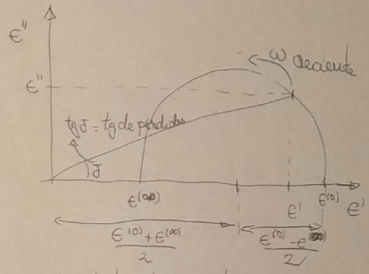
\includegraphics[width=0.4\textwidth]{img/perdidas.png}
    \caption{Circunferencia donde vemos las pérdidas}
    \label{fig:img-perdidas-png}
\end{figure}
El factor $\varepsilon''_{max}$ es el factor de pérdidas, ya que mediante el proceso de relajación se pierde energía. \\
\\
$\tan\left( \delta \right) = \frac{\varepsilon''}{\varepsilon'}=D$ es la tangente de pérdidas\\
\\
$Q=\frac{1}{D}$ es el factor de calidad\\
\\
Pero esto solamente funciona para nuestro modelo. Hay mas
\section{Tema 7: Caracterízación microscópica del magnetismo material}
Pensemos en un electrón orbitando alrededor de un protón. Este electrón tiene un momento orbital asociado:
\[
\vec{l}= \vec{r}\times \vec{p}= -q \vec{R_a}\cdot \vec{v_e}
.\] 
Donde $v_e$ es la velocidad del electrón. \\
\\
El momento dipolar de una espira viene dado por :
 \[
\vec{m}= I\pi \cdot R^2
.\] 
Con estas ecuaciones llegamos a que:
\[
\boxed{\vec{m}= \frac{-e}{2m_e}\vec{l}= -m_B\cdot \frac{\vec{l}}{\hbar }}
.\] 
Vemos que el momento magnético es antiparalelo al momento angular (esto es por la carga negativa del electrón)

\subsection{Parámetros que definen el carácter magnético}
\begin{itemize}
    \item Susceptibilidad: $\chi_m$ : $\vec{M}=\chi_m \vec{H}$
    \item Permeablidad: $\mu_0$
    \item Momento dipolar: $\vec{m}$ 
    \item Intensidad magnética local : $H_L$    
\end{itemize}
\subsection{Modelo de Lorentz}
Definición del vector intensidad magnética:
\[
    \vec{H}= \frac{\vec{B}}{\mu_0}   - \vec{M} = \frac{1}{4\pi}\int_V \frac{\vec{J}\times \left( \vec{r}-\vec{r}' \right) }{ \mid \vec{r}- \vec{r}'  \mid ^3} dV' - \nabla  \varphi^* \left( \vec{r}' \right) 
.\] 
El modelo de Lorentz constiste en calcular el vector intensidad magnética en un punto del medio, donde creamos una esfera imaginaria. Consideraciones:
\[
    \vec{\nabla }\cdot M=0
.\] 
Dentro de la esfera, los dipolos se orientan de forma aleatoria. por tanto:

\[
    \vec{H}=\vec{H_{ext}}+ \vec{H_{int}}= \vec{H}_{mac}^1+ \vec{H}_{mac}^2+ H'
.\] 
Donde $H'=0$ 

\subsection{Origen paramagnetismo}
el orie

\subsubsection{Ley de Curie}
Ley de Curie:
\[
    \chi_{m}= \frac{nm^2\mu_0}{3K_BT}=\frac{C}{T}
.\] 
Esta relación inversamente proporcional entre la susceptibilidad magnética y la temperatura se conoce como la ley de Curie. Esta ley solo es válida para valores bajos de la energía de interacción dipolar magnética con respecto a la energía de equilirbio térmico $\left( K_{B}T \right) $\\
\\
Veamos las diferencias con la polarización por orientación. La principal diferencia es que cuando decimos que un átomo tiene un momento dipolar magnético permanente, tendrá un momento angular permanente ya que:
\[
 \vec{m}= -m_{B}\frac{\vec{l}}{\hbar }
.\] 
Esto deriva de que el electrón tiene tanto carga como masa. Pro tanto, cuando se mueve en órbitas alrededor del núcleo, también es una masa girando. Esto es completamente distinto a la situación de la polarización por orientación donde un momento dipolar eléctrico puede tener una situación estática
\subsubsection{Ley de Curie-Weiss}
Partimos de \[
\vec{m}= -g m_{B}\frac{\vec{J}}{\hbar }
.\] 
\subsection{ferromagnetismo}
Tan solo tiene efecto por el momento angular de spin
\section{Seminarios}
\begin{tcolorbox}[enhanced,attach boxed title to top center={yshift=-3mm,yshifttext=-1mm},
colback=blue!5!white,colframe=blue!75!black,colbacktitle=blue!80!black,
title=Boletin 1,fonttitle=\bfseries,
 boxed title style={size=small,colframe=blue!50!black} ]
 Densidad de carga y corriente con potenciales electromagnéticos:
 \[
     \nabla^2\varphi+\frac{\partial \left( \vec{\nabla} \cdot \vec{A} \right)}{\partial t} = - \frac{\rho_L}{\varepsilon_0} 
 .\] 
 \[
     \nabla ^2A-\mu_0\varepsilon_0 - \vec{\nabla }\left( \vec{\nabla }\cdot \vec{A}+ \frac{1}{c^2} \frac{\partial \varphi}{\partial t}  \right) = -\mu_0 \vec{j}_c  
 .\] 
 Ecuaciones de Maxwell:
 \[
     \vec{\nabla }\cdot \vec{E}= -\frac{\rho_L}{\varepsilon_0}
 .\] 
 \[
     \vec{\nabla }\times \vec{E}= - \frac{\partial \vec{B}}{\partial t} 
 .\] 
 \[
 \vec{\nabla }\cdot \vec{B}=0       
 .\] 
 \[
 \vec{\nabla }\times \vec{B}= \mu_0 \vec{j}_c+ \frac{1}{c^2}\frac{\partial \vec{E}}{\partial t} 
 .\] 
 Condensador placas paralelas:
 \[
 \vec{E}= \frac{\sigma}{\varepsilon_0} \vec{u}_z
 .\] 
 Densidad energía electromagnética:
 \[
     u_{EM}= \frac{1}{2}\left( \vec{D}\cdot \vec{E}+\vec{B}\cdot \vec{H} \right) \implies U_{EM}=\int_V u_{EM}dV
 .\] 
 Vector de Poynting:
 \[
 \vec{S}=\vec{E}\times \vec{H}
 .\] 
 Ecuación de continuidad:
 \[
     \frac{d U_{EM}}{dt} = \oint \vec{S}d\vec{\Sigma}
 .\] 
Tensor de esfuerzos de Maxwell:
\[
\frac{d \vec{P}_{mec}}{dt} + \frac{d\vec{G}}{dt} = F_q= \varepsilon_0\oint \overline{T}\cdot d\vec{S}
.\] 
Tensor de esfuerzos:
\[
    \oint \overline{T}\cdot d\vec{S}; \;\;\;\overline{T}=\overline{T_e}+ \overline{T_m};
.\] 
\[
    \oint \left( \left( \vec{E\cdot \vec{n}} \right) \vec{E}-\frac{1}{2}E^2\vec{n} \right) d\vec{S}
.\] 
Diferencial de superficie en cilíndricas:
\[
d\vec{S}= \rho d\rho d\phi = 2\pi \rho d\rho
.\] 
\[
    \phi = [0,2\pi]
.\] 
\[
\rho=[0,R]
.\] 
\end{tcolorbox}

\newpage
\begin{tcolorbox}[enhanced,attach boxed title to top center={yshift=-3mm,yshifttext=-1mm},
colback=blue!5!white,colframe=blue!75!black,colbacktitle=blue!80!black,
title=Boletín 2,fonttitle=\bfseries,
 boxed title style={size=small,colframe=blue!50!black} ]
 Conductor real:
 \[
     K_2=\alpha - j\beta = \sqrt{\frac{\omega \mu_0 \sigma}{2}} - j \sqrt{\frac{\omega \mu_0 \sigma}{2}}= \left( \frac{1-j}{\delta} \right) ; \;\;\;\; \delta= \sqrt{\frac{2}{\omega  \mu_0 \sigma}} 
 .\] 
\end{tcolorbox}
\[
k_2
.\] 

\section{Nuevo Tema}%
\label{sec:Nuevo Tema}
hola 


%\input{tex/circuitos}
%\chapter{Física CuánticaI}%
\section{Tema 1: Historia Física Cuántica}%

%	Comienza la inclusión de cada tema
\chapter{Electromagnetismo I}
\section{Tema 1: Campo eléctrico}
%	Tema 1: Campo eléctrico
\[
	\vec{E}\left( \vec{r} \right) =\frac{q}{4\pi \epsilon_0}\sum_{n=1}^{N} \frac{\vec{r}-\vec{r'_i}}{ \mid \vec{r}-\vec{r'_i} \mid ^3}
.\] 

%\chapter{Mecánica De Medios Continuos}

%\chapter{Física Estadística}


%\chapter{Física Cuántica I}



\appendix
\end{document}

